\documentclass[parskip=half,DIV=16]{scrartcl}

\title{Project report}
\subtitle{ATM S 544}
\author{Dominik Stiller}
\date{\today}

\usepackage[english]{babel}
\usepackage[utf8]{inputenc}
\usepackage{siunitx,amsmath,physics}
\usepackage{caption,subcaption,graphicx,csquotes,xcolor}
\usepackage{booktabs}
\usepackage{placeins}
\usepackage[
	backend=biber,
	bibwarn=true,
	bibencoding=utf8,
	sortlocale=en_US,
	url=false,
	style=apa,
	isbn=false
]{biblatex}

\definecolor{uw-purple}{RGB}{51, 0, 111}

\usepackage{hyperref}
\hypersetup{
	% hidelinks,
	colorlinks=true,
	linkcolor=black,
	citecolor=black,
	urlcolor=uw-purple
}

\usepackage{doi}
\usepackage{nomencl}
\makenomenclature
\usepackage[noabbrev,capitalise]{cleveref}
\usepackage[acronym,nonumberlist,nopostdot,nogroupskip]{glossaries}
\usepackage[
	outputdir=build,
]{minted}
\setminted{
	linenos,
	tabsize=4,
	fontsize=\small,
}
\newmintinline{python}{}

\usepackage{lmodern}
\usepackage[T1]{fontenc}
\usepackage{inconsolata}
\usepackage{tikz}

\newcommand{\result}[1]{\colorbox{uw-purple}{\textcolor{white}{#1}}}

\setlength{\nomlabelwidth}{1.5cm}
\setlength{\nomitemsep}{-\parsep}
\newcommand{\nomunit}[1]{%
\renewcommand{\nomentryend}{\hspace*{\fill}\si{#1}}}

\sisetup{per-mode=symbol}
\AtBeginDocument{\RenewCommandCopy\qty\SI}

\DeclareGraphicsRule{.ai}{pdf}{.ai}{}

\addbibresource{bibliography.bib}


\makeglossaries
\newacronym{LIM}{LIM}{linear inverse model}
\newacronym{DA}{DA}{data assimilation}
\newacronym{EOF}{EOF}{empirical orthogonal function}
\newacronym{EnSRF}{EnSRF}{ensemble square-root filter}


\begin{document}

\maketitle


\section{Introduction}

For this project, I reproduced some results of \textcite{Perkins2021}\footnote{The three Perkins \& Hakim papers are hereafter referred to as PH17, PH20, and PH21.}, who reconstructed ten climate fields over the last millennium. Their paleoclimate \gls{DA} method combines the ensemble forecast of a coupled ocean--atmosphere \gls{LIM} with proxy observations by means of an \gls{EnSRF}. Since I will continue this line of research, my project is less concerned with originality and more with familiarizing myself with the data, methods, and workflow.

There are some notable differences of my implementation compared to PH21:
\begin{itemize}
    \item They use training data for the \gls{LIM} from CMIP5 \emph{past1000} simulations, while I use CMIP6 \emph{past2k} experiment data. Therefore, my training dataset is larger and more recent.
    \item They use real proxy observations from the Pages2k, while I generate noisy pseudo-observations from a CMIP6 \emph{past1000} simulation.
    \item They validate against instrumental datasets, while I validate against the simulation from which the pseudo-observations are drawn.
\end{itemize}
Note that using pseudoproxies and verifying against their "truth" allows me to check the correctness of my code rather than actually reconstructing the past climate.

My \gls{LIM} training dataset is the \emph{past2k} simulation~\parencite{Jungclaus2017}, which models 400 coupled ocean--atmosphere fields over 1--1849 CE at monthly resolution. The extended simulation compared to the \emph{past1000} experiments allows better investigation of the medieval period; the forcings and spin-up are identical to the shorter variant. For us, the benefit are 850 additional years to learn ocean--atmosphere dynamics from. I used the \emph{past2k} simulation of the MPI-ESM1-2-LR model, which is the only available one.




\section{Forecasting and data assimilation setup}

\begin{figure}[h]
    \centering
    \includegraphics[width=0.8\textwidth]{figures/architecture.ai}
    \caption{Setup for cycling \gls{DA}.}
    \label{fig:arch}
\end{figure}

The main components of my reconstruction code are shown in \cref{fig:arch}. A mapper translates between the high-dimensional physical space for \gls{DA} and the low-dimensional space for forecasting (\cref{subsec:setup-dimred}). The \gls{LIM} provides an ensemble forecast based on initial conditions in this reduced space (\cref{subsec:setup-lim}). Observations are assimilated in the physical space by the \gls{EnSRF} (\cref{subsec:setup-ensrf}). This section describes the technical aspects of my cycling \gls{DA} setup.


\subsection{Dimensionality reduction for LIM}
\label{subsec:setup-dimred}

The \emph{past2k} simulation output of MPI-ESM1-2-LR contains $\sim$400 fields on its native grid of \qtyproduct{1.875 x 1.875}{\degree}. Like PH21, I regridded the data to a regular \qtyproduct{2.0 x 2.0}{\degree} latitude--longitude grid using bilinear interpolation and select ten fields: 2 m surface air temperature (tas), precipitation (pr), sea-level pressure (psl), 500 hPa geopotential height (zg500), outgoing top-of-atmosphere longwave radiation (rlut), reflected top-of-atmosphere shortwave radiation (rsut), sea-surface temperature (tos), sea-surface salinity (sos), dynamic ocean surface height (zos), and \qtyrange{0}{700}{m} ocean heat content (OHC700). I then formed annual averages from April to March since many real proxies do not have higher temporal resolution. This also means that the \gls{LIM} forecast step is 1 year.

The original state vector for each timestep is 162 000-dimensional, even after regridding and field selection, which poses a large computational burden for the \gls{LIM}. PH21 leveraged joint modes of variability to reduce the state to 50 dimensions while retaining sufficient variance. The dimensionality reduction comprises multiple steps:
\begin{enumerate}
    \item Mask out nan values. These do not have to be included in the state vector. For example, ocean fields do not have values over land, and I needed to remove some spurious invalid values, particularly above the poles.
    \item Remove trend. The \gls{LIM} assumes stationary statistics~\parencite{Penland1995} and forecasts anomalies; removing the trend yields these anomalies.
    \item Fit and project each field individually onto \glspl{EOF}. PH21 found that 400 components retain more than 90\% of each fields variance. Each grid cell is latitude-weighted before fitting the \glspl{EOF}.
    \item Standardize each field individually. (The pr field is standardized before EOF projection since its small magnitude makes it prone to numerical noise.)
    \item Stack all fields except ohc700, then fit and project them onto a joint \gls{EOF}. I retain the leading 30 components, slightly more than PH21 since my data are different. This highlights how coupled field variability really is.
    \item Truncate the ohc700 field to 20 components. This field is kept separate because its dynamics are much slower than the other fields, particularly atmospheric ones.
    \item Stack the 30 joint EOF components and 20 ohc700 components into a single 50-dimensional vector.
\end{enumerate}
To map back into physical space, these steps are applied in reverse order. The dimensionality reduction compresses the ten fields from 26 GB down to just 1 MB (a factor 12 of which is due to the annual averaging)/

\begin{figure}[h]
    \centering
    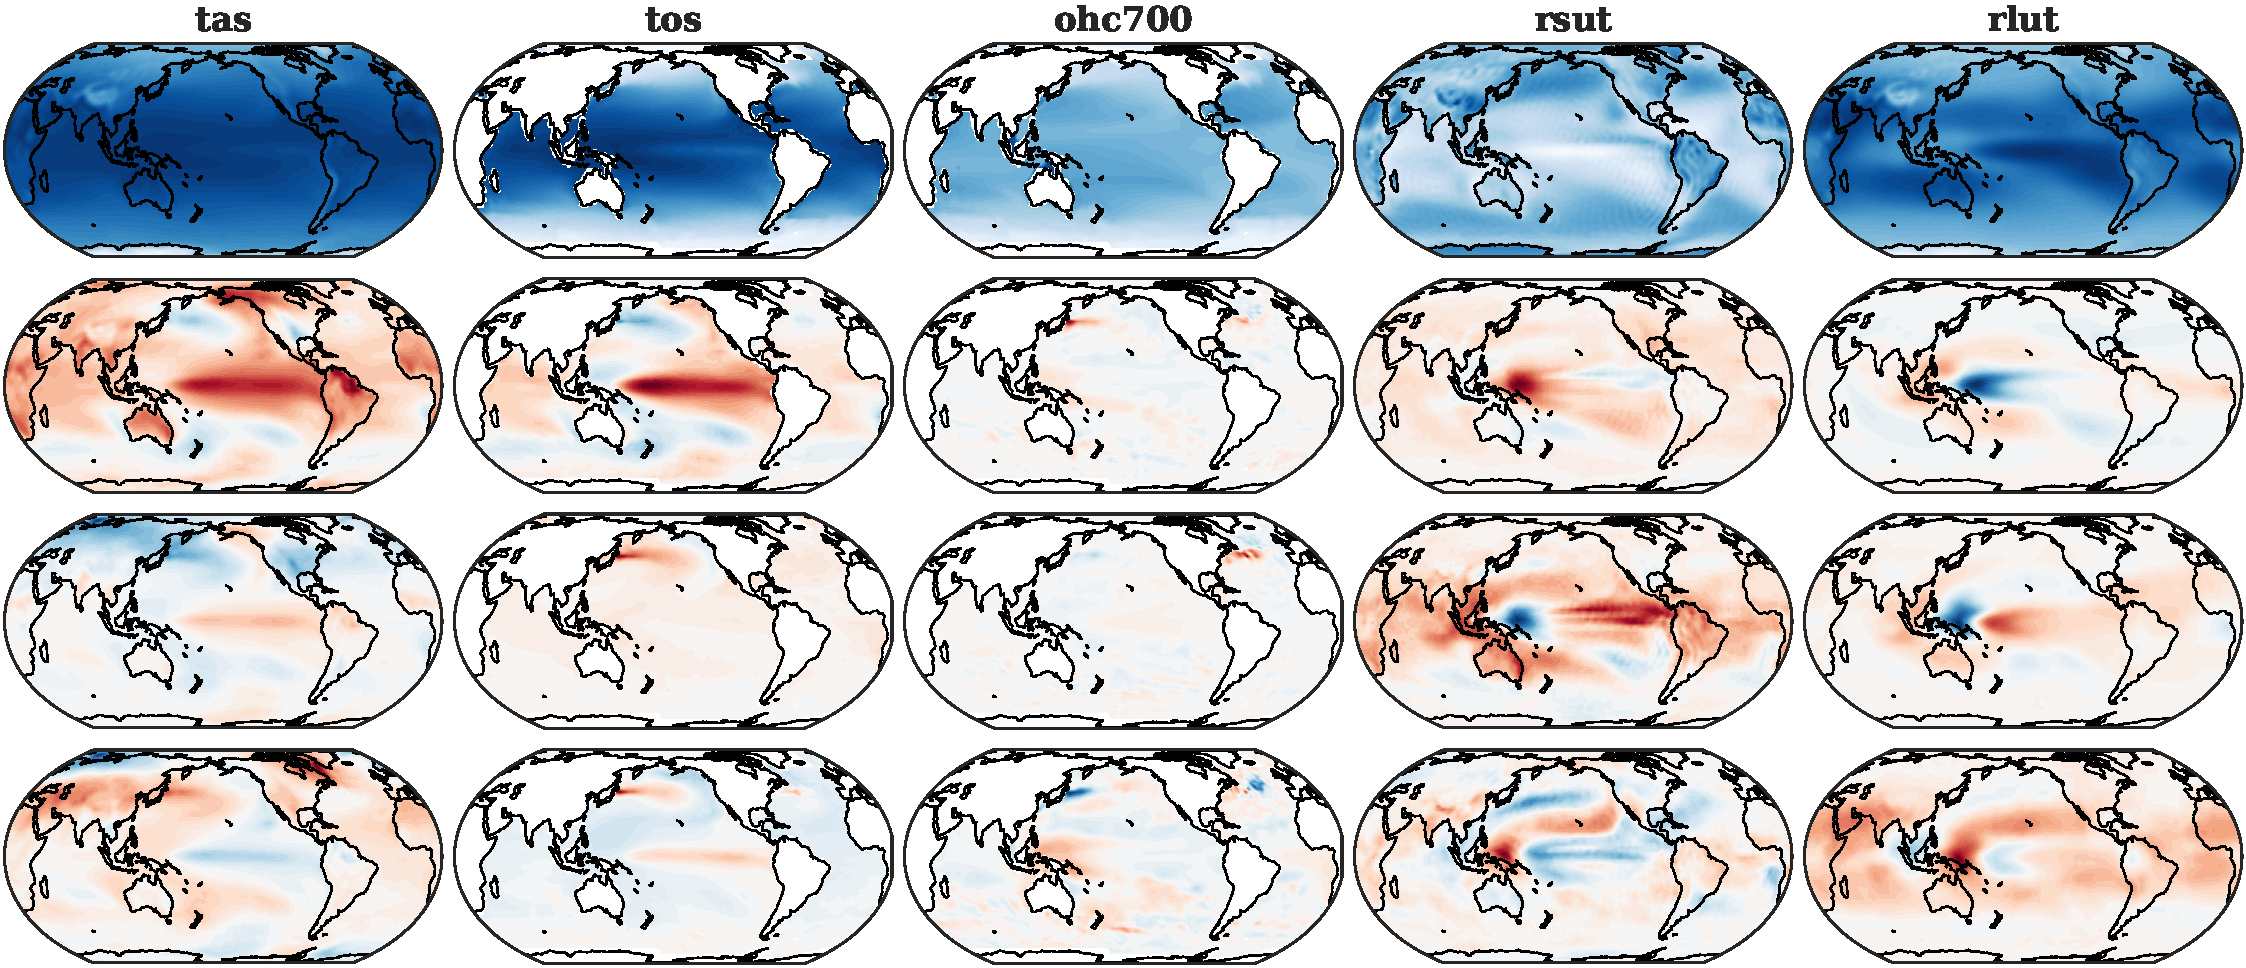
\includegraphics[width=\textwidth]{figures/plots/eofs.pdf}
    \caption{Mean (top) and first three \glspl{EOF} (below) for a selection of fields.}
    \label{fig:eofs-mine}
\end{figure}

\cref{fig:eofs-mine} shows the mean and leading \glspl{EOF} that my code found. All of them look physical (as far as I can judge) and show well-known patterns such as ENSO and the Indonesian Throughflow. The ohc700 field is clearly distinct with less spatial variability. This supports its separate treatment in the reduction procedure.

\begin{figure}[h]
    \centering

    \begin{subfigure}[c]{0.3\textwidth}
        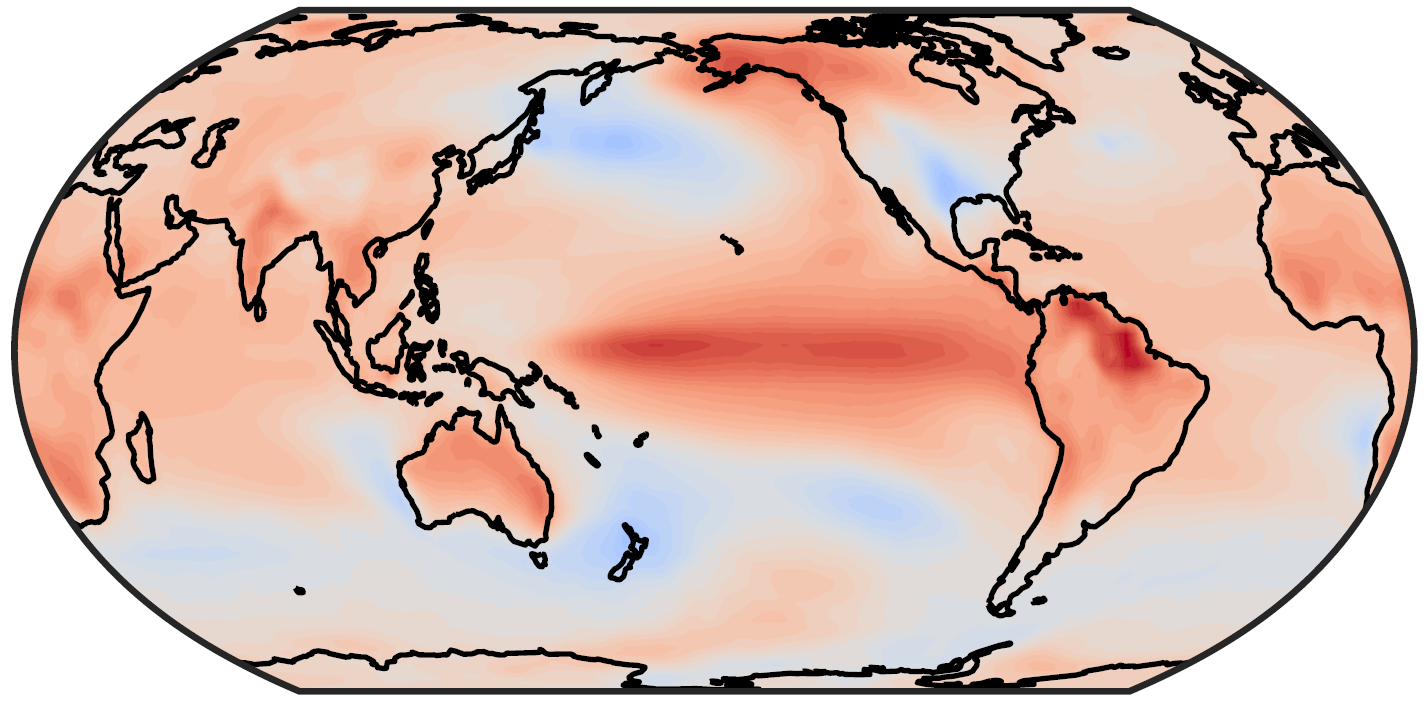
\includegraphics[width=\textwidth]{figures/eoftas_mine.png}
        \subcaption{Mine (CMIP6 MPI)}
     \end{subfigure}
     \hfill
     \begin{subfigure}[c]{0.3\textwidth}
        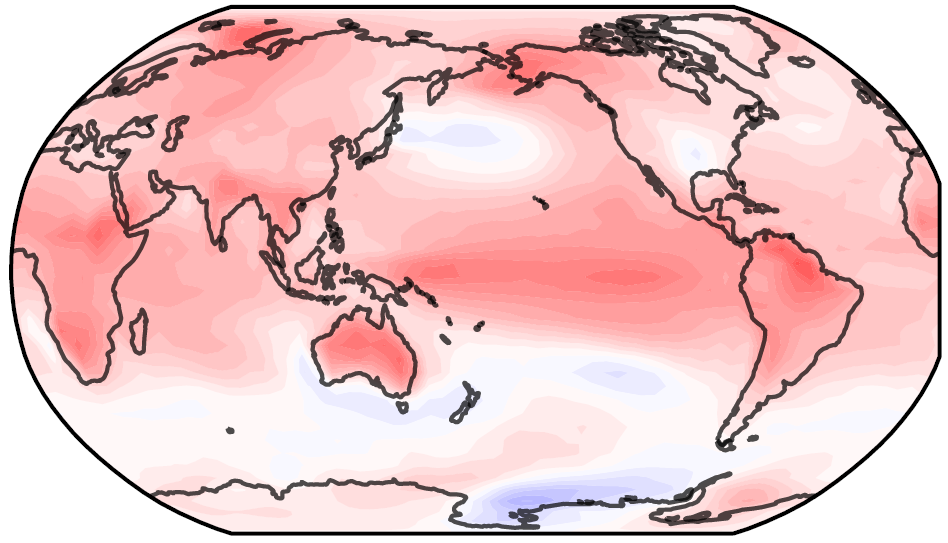
\includegraphics[width=\textwidth]{figures/eoftas_ph17_mpi.png}
        \subcaption{PH17 (CMIP5 MPI)}
     \end{subfigure}
     \hfill
     \begin{subfigure}[c]{0.3\textwidth}
        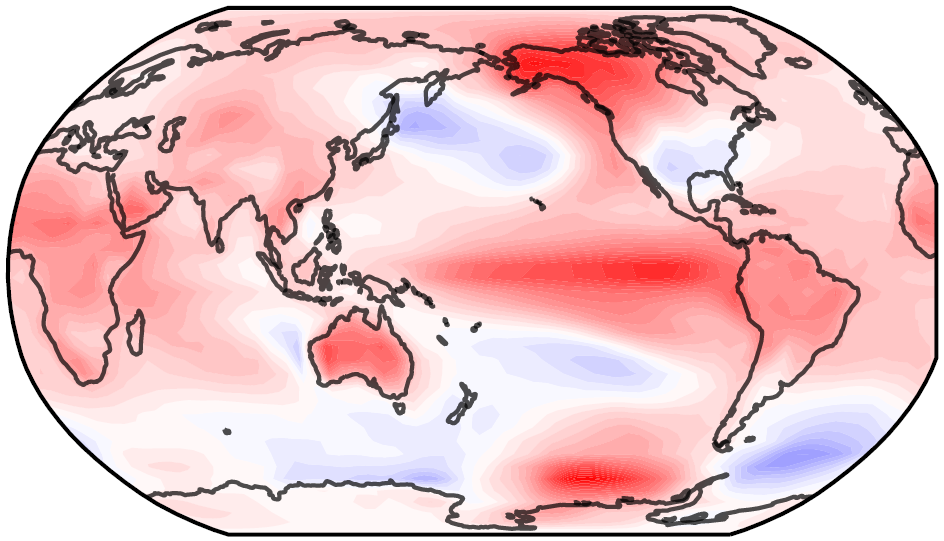
\includegraphics[width=\textwidth]{figures/eoftas_ph17_ccsm.png}
        \subcaption{PH17 (CMIP5 CCSM)}
     \end{subfigure}

    \caption{Leading EOFs for TAS from my and \textcite{Perkins2017} (PH17) reconstructions.}
    \label{fig:eofs-ph}
\end{figure}

We can compare the leading \gls{EOF} of tas (first column, second row in \cref{fig:eofs-mine}) to those found by \textcite{Perkins2017} in \cref{fig:eofs-ph}. Their \glspl{EOF} are derived from CMIP5 \emph{past1000} outputs of the CCSM and MPI models while mine comes from the CMIP6 version of the MPI model. The patterns are generally similar: a pronounced warm pattern in the tropical Pacific is flanked by colder regions; hot Australian and North American continents. The Southern Ocean and South America regions show more similarity between the MPI models, but the North Pacific low is smaller in the CMIP5 MPI version. Still, the \glspl{EOF} are similar enough for us to conclude that the choice of training data has little effect on the TAS reconstructions.



\subsection{LIM for forecasting}
\label{subsec:setup-lim}

The \gls{LIM} is an efficient forecast model that makes online \gls{DA} computationally feasible. The forecast allows information to be propagated through time, particularly by inclusion of ohc700, which acts as dynamic memory to inform low-frequency variability. In addition, the cheap forecasting enables large ensembles: forecasting my 100 ensemble members takes less than 1 s.

A \gls{LIM} can represent a linear system of the form
\begin{align*}
    \dv{\vb{x}}{t} = \vb{L}\vb{x} + \vb*{\xi},
\end{align*}
where $\vb{L} \in \mathbb{R}^{N_x \times N_x}$ is a linear operator and $\xi \sim N(0, \vb{Q}/dt)$ is additive Gaussian noise. In my case, the state dimension is $N_x = 50$. The deterministic forecast equation is then~\parencite{Penland1995}
\begin{align*}
    \vu{x}_{k+1} = \exp (\vb{L} \, \Delta t) \, \vb{x}_k  = \vb{G} \vb{x}_k ,
\end{align*}
where $\vb{G} \in \mathbb{R}^{N_x \times N_x}$ is the linear forecast operator. For probabilistic ensemble forecasts, we can use the two-step stochastic integration scheme proposed by \cite{Penland1994}:
\begin{align*}
    \vb{x'}(t+\delta t) &= \vb{x'}(t) + \vb{L}\vb{x'}(t) \, \delta t + \vu{Q} \sqrt{\vb{\Lambda}\delta t} \mathcal{R},
    \\
    \vb{x}(t + \delta t / 2) &= \left[\vb{x'}(t) + \vb{x'}(t+\delta t)\right] / 2,
\end{align*}
where $\vu{Q}$ and $\vb{\Lambda}$ come from the eigendecomposition $\vb{Q} = \vu{Q} \vb{\Lambda}\vu{Q}^{-1}$ of the noise covariance matrix and $\mathcal{R}$ is a vector of random numbers drawn from a standard normal distribution. The integration timestep $\delta t$ must be chosen much smaller than the corresponding deterministic timestep $\Delta t$. PH21 use $\delta t \approx \qty{6}{h}$, which requires 1440 integration steps over a period of $\Delta t = \qty{1}{year}$.

The system dynamics $\vb{L}$ and $\vb{G}$ as well as the noise covariance $\vb{Q}$ can be determined from data. The procedure is based on the zero-lag and $\tau$-lag covariance matrices:
\begin{align*}
    \vb{C}(0) = \langle \vb{x}(t) \vb{x}^\transpose*(t) \rangle \qquad \mathrm{and} \qquad \vb{C}(\tau) = \langle \vb{x}(t+\tau) \vb{x}^\transpose*(t) \rangle,
\end{align*}
where $\langle \cdot \rangle$ denotes the time average. In my case, the average is over 1848 timesteps (one year is removed by the split-year annual average, another by the 1-year lag). The forecast operator is then recovered as
\begin{align*}
    \vb{G} = \vb{C}(\tau) \vb{C}(0)^{-1}.
\end{align*}
This reveals $\vb{G}$ to be the sensitivity between the state at $\tau$-lagged timesteps, normalized by the state covariance. The linear operator $\vb{L}$ required for stochastic integration is then found as
\begin{align*}
    \vb{L} = \frac{\ln\vb{G}}{\tau}.
\end{align*}
The logarithm is preferably evaluated by eigendecomposition of $\vb{G}$. Finally, we can find the noise covariance matrix as
\begin{align*}
    \vb{Q} = - \left( \vb{L} \vb{C}(0) + \vb{C}(0) \vb{L} \right).
\end{align*}
While covariance matrices are positive semi-definite, the $\vb{Q}$ found here may have spurious negative eigenvalues as a result of a short training period or significant non-linear dynamics~\parencite{Penland1994}. We can remove these negative eigenvalues by eigendecomposition of $\vb{Q}$, but have to rescale the remaining ones to retain the total variance.



\subsection{EnSRF for data assimilation}
\label{subsec:setup-ensrf}

The ensemble forecast from the \gls{LIM} requires a \gls{DA} scheme that is compatible with ensemble priors. For simplicity, I use the \gls{EnSRF}~\parencite{Whitaker2002} also employed in PH17, while PH21 use an ensemble transform Kalman filter. The results should be similar if not identical between the two. I did not have time to implement covariance localization and calibrate my filter through inflation or additive noise.

The \gls{EnSRF} works on the assumption that observations are independent so that Bayes' rule can be applied sequentially. First, the ensemble is converted into perturbations
\begin{align*}
    \vb{X} = \mqty[ \vb{x}^{1} - \vu{x} &  \vb{x}^{2} - \vu{x} & \ldots &  \vb{x}^{N_e} - \vu{x} ],
\end{align*}
where $\vb{x}^i$ are the ensemble priors (column vectors) and $\vu{x}$ is their mean. In my case, the number of ensemble members $N_e = 100$. We then define the ensemble prior of the observations
\begin{align*}
    \vb{Z} = \vb{H} \vb{X},
\end{align*}
which allows us to efficiently compute the variance of the observation forecast as
\begin{align*}
    \hat{\sigma}_p^2 = \frac{\vb{Z} \vb{Z}^\transpose}{N_e-1}.
\end{align*}
The analysis ensemble perturbations are then
\begin{align*}
    \vb{X}^a = \vb{X} \left( \vb{I} - \alpha \frac{\vb{Z} \vb{Z}^\transpose*}{(N_e-1)(\hat{\sigma}_p^2 + \sigma_o^2)} \right),
\end{align*}
where $\sigma_o^2$ is the observation variance. Notice that the analysis perturbations must be in the span of the prior perturbations. The scalar $\alpha$ such that the analysis covariance is correct is found as
\begin{align*}
    \alpha = \left( 1 + \sqrt{\frac{\sigma_o^2}{\hat{\sigma}_p^2 + \sigma_o^2}} \right)^{-1}.
\end{align*}
Next, we compute the analysis ensemble mean as
\begin{align*}
    \vu{x}^a = \vu{x} + \frac{\vb{X}\vb{Z}^\transpose}{(N_e-1)(\hat{\sigma}_p^2 + \sigma_o^2)} \left( y - \vb{H} \vu{x} \right).
\end{align*}
Finally, we combine mean and perturbations to form the posterior ensemble
\begin{align*}
    \left(\vb{x}^i\right)^a = \vu{x}^a + \vb{X}^a_i,
\end{align*}
which is the initial condition for the next forecast of the \gls{LIM}.




\subsection{Setup for cycling data assimilation}

For this project, I only reconstruct over 850-1050 CE due to time constraints. I fitted the physical--reduced space mapper on the Casper cluster, which produced the training dataset for the \gls{LIM}. The remaining steps (fitting the \gls{LIM}, running the reconstruction, analyzing the results) were performed on Greg's \texttt{enkf} server.

\begin{figure}[h]
    \centering
    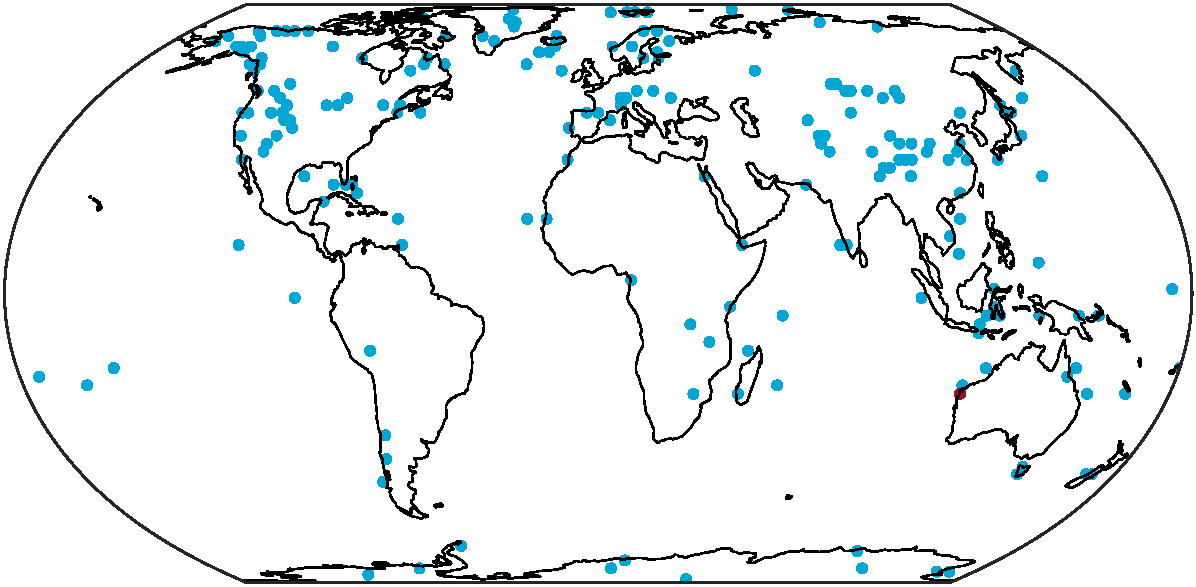
\includegraphics[width=0.5\textwidth]{figures/plots/obs_locations.pdf}
    \caption{Pseudo-observation locations.}
    \label{fig:obs-locs}
\end{figure}

My ensemble has 100 members, which are initialized from a random draw of 1000 years from the training dataset. My pseudo-observations come from annual averages of the CMIP6 \emph{past1000} output of the MRI-ESM2-0 model. Drawing them from a different model than the training data should lead to a more challenging testbed for my \gls{DA} system. The observations are surface air temperatures from locations of the Pages2k proxies~\parencite{PAGESConsortium2017}, which is the real dataset used by PH21. I draw a random sample of 200 locations (the same ones for every year of the reconstruction), which is about average of the number of proxies assimilated per year in PH21 over the whole last millenium. The 200 locations are shown in \cref{fig:obs-locs}. The pseudo-observations are perturbed by Gaussian noise with $\sigma_o^2 = \qty{1}{K^2}$, which is also the variance used in the \gls{EnSRF}.




\section{LIM results}


also show heatmap for Q matrix



\section{DA results}

compare to MRI model as validation

For reconstructed GMST plot: show LIM free run, LIM + DA, training data
s

use area-weighted GMST



\subsection{Sanity check}
variance should decrease
posterior should be between prior and obs


\printbibliography


\end{document}
